
\documentclass[conference]{IEEEtran}


\begin{document}
	
\title{Importance of Cooperative gameplay in Multiplayer online battle arena (MOBA) games}


\author{\IEEEauthorblockN{Gautam Baghel, Magy Seif El-Nasr}
\IEEEauthorblockA{College of Computer and Information Science\\
Northeastern University\\
Boston, Massachusetts 02115\\}

}

\maketitle

\begin{abstract}
Computer game contributes a huge part to modern culture. Among different types of computer games, the multi-player online battle arena games generated an electronic sports community and attracted plentiful audiences. LOL (League of Legends), as one of the leading multi-player online battle arena games, Riot has a big responsibility on analyzing game data and improving game experiences to players. This paper applies classification methods to identify the contribution of teamwork performance and star player performance to winning. Through various methods verification, the results show using teamwork behavior has higher prediction accuracy than using one-star player performance data in a match. In sum, the results with a data set of 534398 team data in 2015 recommend better teamwork contributes more to winning than single star player performance.
\end{abstract}

\IEEEpeerreviewmaketitle



\section{Introduction}

In recent years, there is a rise in popularity of MOBA (Multi-Player Online Battle Arena) games. These games are usually composed of several players forming teams and competing against each other in matches. Each match can range from few minutes of play to hours of play. League of Legends alone reportedly has over 100 million monthly active users \cite{Loterina}. Professional players have made careers out of playing professional MOBA games with earnings in the range of two million dollars annually \cite{esports}. Electronic sports (eSports) are becoming an important part of our culture. In this paper, we are interested in (a) understanding how teamwork is established within a team and how that may impact win/loss. Understanding if the team is important rather than just one player which means more engagement to all the team rather than them relying upon one has design and user experience implication, but also perhaps a learning implication. For game designers, it may be environmental elements of the game which contribute to synergy in a game. For producers, it may be involvement of more players and getting them hooked on the game. For players, it gives them an opportunity to refine their skills where it proved to be inadequate.

To achieve this goal, the paper uses a game analytics approach where data from a MOBA game is analyzed through machine learning algorithms. There has been similar work in this area. Looking at several aspects of team composition from player personalities to champion types in the game. Player personalities may vary in different players altogether and the findings are preliminary. Champion type analysis only looks at the composition based on champion specific skills, player effectiveness in using the champion is not evident. Team versus star player analysis gives a better picture of cooperation versus competition in the game.  

In order to tackle this problem, we analyzed 534,398 data of team statistics from MOBA game. We used analyzed the team vs. star player on the team in terms of their contribution to winning/losing. To answer that we turned this into a classification question where we predict win/loss based on team features vs. star-player features. This kind of analysis is the first of its kind to understand the contribution of team members and features influencing win/loss from different team members. The contribution is in the results that we found and it adds to previous work on team level analysis in MOBA game from a different perspective. 

This paper is divided into the following section. First, we discuss previous work in more detail outlining the open problems given the work done in MOBA games. Second, we discuss the game we used and the dataset. Third, we discuss the algorithms used and results obtained. We then discuss the results in more detail. We conclude by outlining the contribution and applications of the results.  



\section{Previous Work}
A study by Christoph Eggert and team \cite{Eggert2015} which classified players into sets of classes and segments of games with respect to their roles, effectiveness in time (early/late) and support items/ damage types. Using Logistic Regression, Random Forest and Bayesian Networks to reduce the set of player classes for better accuracy in predicting the winner. A team-based approach to MOBA is similar but on aspects divided on roles. Limitations may include predetermining roles in the game which may lead to some early misdirection in team formation.

 Personality aspects have also been taken into consideration while forming a team where the study investigated how personality trait and expertise affect virtual team interactions \cite{Balthazard2004}. Using correlation analysis, regression analysis, and a series of post hoc t-tests they were able to hypothesize the mechanisms through which personal characteristics of individuals are aggregated via group-level dynamics to produce group-level outcomes and approached the  team v/s individual performance based on personality traits. They concluded that the results were preliminary and since they were formed into interdependent teams for only the relatively brief duration of their task it cannot be used universally.

Another team analysis 'Learning Dota 2 Team Compositions' \cite{Agarwala2014}, studied teams using PCA and second order PCA with Logistic regression was done for a different MOBA game Dota 2, using hero composition. They concluded that cleaner data or better models are needed. Factors responsible may have been player skills which were not taken into consideration.

The clustering algorithm used in the paper Player Behavior and Optimal Team Composition based on champion types is done in Online Multiplayer Game study based on champion types by Hao Yi Ong and team \cite{Bainbridge2009} was effective in forming teams based on champion types. The focus in this paper is on player types like ambush-er, magic, physical, support etc. and team composition from that, whether a specific class of champions has any effect on winning. It uses clustering of players based on their behaviors, visualizing the data using PCA and predicting the winner using classification. Factors not taken into consideration was team play behaviors like assists and player skill-based classification.

Research done in similar area  Player Skill Decomposition in Multiplayer Online Battle Arenas \cite{Chen2016} looked at 14 cooperative games to find out game-play design aspects which determine the interaction between player. Their research showed that helping occurred when the game was difficult for players which may be a factor in teams which win in the league of legends. Results may be time dependent and as the game changes rapidly over the years, player strategies may have evolved differently from MOBA games. 

Making use of game log data, 'On Successful Team Formation' \cite{Pobiedina2013b} chose a statistical approach to identify factors that increase the chance of a team to win. Their hypothesis being better role distribution in a team increases the chance to win a game,     teams with more experienced players have a higher chance to win, playing with friends increases the chance to win and
the selection of a proper leader as well as a good matching of heroes inside a team positively influence the success. Using ANOVA test and Mann-Whitney-Wilcoxon-tests they were able to identify better Individual Hero Selection vs Team Hero Selection with log-linear analysis. In this approach, specific Gameplay elements not considered the part of analysis since MOBAs tend to be different from other online multiplayer games where gameplay aspects like inhibitors, dragons are quintessential to form strategies it falls short.
  
Effectiveness of Machine Learning algorithms in predicting game outcome by systematic review and compare performance of most frequently used machine learning algorithms for prediction of the match winner from the teams' drafts in DotA 2 computer game \cite{Semenov} deals with algorithms such as Naive Bayes classifier, Logistic Regression and Decision trees to validate consistency in data mining. Using the algorithms this paper comes up with standard performance metrics for players. This paper deals with different algorithms than the ones previously presented.

\section{Game and Data}
The data set consists of about two million League of Legends (LOL) matches that happened in 2015 summer retrieved using riots API system. The game mode is called 5-vs-5 ranked matches of a solo queue which is extensively played MOBA mode. A typical such match involves ten players who form two teams of five. Each match consists of ten rows with statistics of each player as shown in (Fig. \ref{fig_sim}). Star player and team data set are segregated which will consist of two rows per match. In the Star player data set, a player who falls under the category of the star player will be placed on each team and in the team data set aggregate of all the player from each team will make two rows per match.


\begin{figure}[!t]
%\centering
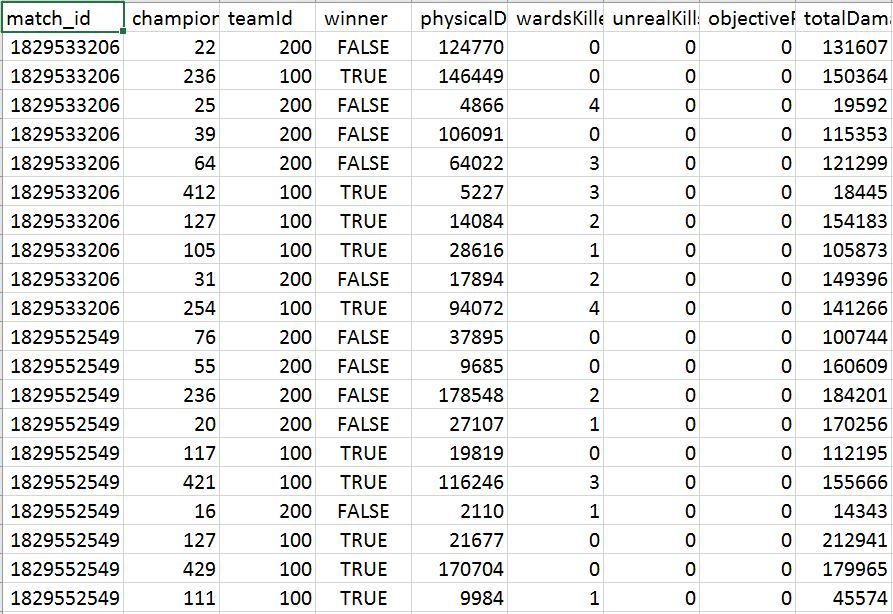
\includegraphics[width=\linewidth]{tab6}
% where an .eps filename suffix will be assumed under latex, 
% and a .pdf suffix will be assumed for pdflatex; or what has been declared
% via \DeclareGraphicsExtensions.
\caption{Dataset with retrieved from riot's API}
\label{fig_sim}
\end{figure}


\section{Feature Extraction}
We derived several features from the given data above: 
\begin{itemize}
  \item \textbf{Star Player}  Using backward feature selection which includes all the predictors and recursively removes the predictors which are less influential, goldEarned was the most important predictor with Akaike information criterion that overrules other predictors. The findings here were corroborated in the heat map of the predictors show that gold earned supersedes every other predictor by huge margins \cite{Patterson}. 
  \item \textbf{Team features}  A similar approach is made as with the star player analysis. Using backward feature selection on assist components of the game which reduces to totalDamageDealt, firstTowerAssist, firstBloodAssist, assists, and firstInhibitorAssist. 
\end{itemize}

\section{Team Features vs. Star Player affecting Win/Loss in Moba Game}


We considered and compared several methods to predict the effect of team vs. star player as features for predicting win/loss. 
After the separation of data set into two distinctive halves, we tried to form a learning model based on the features. The datasets comprised of categorical and quantitative data so every algorithm used had its pros and cons. When choosing reasonable methods, some dimensions are considered. For example, the number of training examples, the feature space dimensionality, the relationship between features, the linearly dependent expiations between features and target variable (winner), the problem of overfitting and the computer system’s capacity on running data analysis. Based on the dimensions we considered, these five models were chosen.

\begin{itemize}
  \item \textbf{Logistic Regression}
We chose this method due to we expect the LOL data features are roughly linear and the hypothesis problem to be linearly separable. This method is also efficient. Also, since LR output can be interpreted as a probability, it is good for predicting winning or losing. 

  \item \textbf{Linear Discriminant Analysis }
Also known as Fisher Linear Discriminant (FLD), is a classical algorithm for pattern recognition. It is an effective feature extraction method. Using this method, the inter-class scatter matrix of the post-projection pattern samples can be maximized, and the intra-class scatter matrix is minimized. In other words, it can guarantee the smallest-in-class distance and the largest inter-class distance in the new space, that is, the pattern can be best separated in that space. However, LDA is not effective when sample information is dependent on variance rather than mean.

  \item \textbf{Quadratic Discriminant Analysis }
LDA requires an assumption of equal variance-covariance matrices between the input variables of the classes. QDA is a modification of LDA which allows for the above heterogeneity of classes' covariance matrices. Since in our team dataset we can't be sure whether the covariance of each of the classes is identical or not it is a good idea to use QDA as well. And it can be used to build the model for more problems. The difference is, when the covariance matrices of different categorical samples are the same, LDA should be chosen. Otherwise, QDA should be used. The reason we use both LDA and QDA is to test which method works better on our problem.

  \item \textbf{Regression Tree}
A Decision Tree (DT) is a graph that uses a branching method to illustrate every possible outcome of a decision. Generally, DT is easier to understand and be explained to most people. Since DT is nonparametric, no worry is needed about whether the data and the outliers are linearly separable. DT’s main drawback is that it is easy to over-fit, which makes the random forest (Random Forest, RF) (or Boosted tree) and other integrated learning algorithm arise. The R package we use is rpart. It solves the over-fitting problem through prune method. It firstly builds a complicated tree model and then estimates the error of each model under different” pruning” conditions according to the Cross-Validation method. This model may prove better as our dataset may contain lots of outliers especially when we analyze the star player. Also, it is useful for our data to be explained in a straightforward way.

  \item \textbf{Clustering}
Another approach is based on unsupervised learning which is different from all the models used above.In clustering we do not train the data set to predict winning, we simply form groups of players with similar characteristics in terms of being a star player or team player. We’ll use our initial training set without segregating it into teams and star players. K-means is a clustering algorithm which tries to form initial cluster centroids and proceeds by repeating cluster assignments and updating centroids. These steps are performed until the algorithm converges. Using the k-means clustering method we’ll append each player a cluster number to which they belong. 
So the dataset currently looks like in Fig. 3.


 K-means starts with a random choice of cluster centers and needs the number of clusters to be specified we have to plot and see the number of clusters appropriate for the analysis.

\begin{figure}[!t]
%\centering
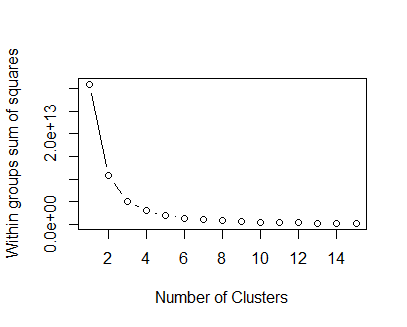
\includegraphics[width=\linewidth]{tab4}
% where an .eps filename suffix will be assumed under latex, 
% and a .pdf suffix will be assumed for pdflatex; or what has been declared
% via \DeclareGraphicsExtensions.
\caption{K-means clustering options}
%\label{fig_sim}
\end{figure}

 From the Fig. 4, five seems to be a good enough cluster choice. At this point, every player in the game will be in a cluster between 1 and 5. For the team analysis now every team will have a score between 5 and 25 by doing the cluster number aggregation. From this number we’ll predict the winner. As the predictors are in higher dimension we’ll use PCA to visualize the data point and which classification method to use. PCA involves all the predictors which constitute to a cooperative gameplay like assists,totalDamageDealt,firstTowerAssist etc. The data points can be seen in Fig. 5.

\begin{figure}[!t]
%\centering
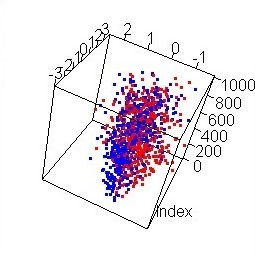
\includegraphics[width=\linewidth]{tab5}
% where an .eps filename suffix will be assumed under latex, 
% and a .pdf suffix will be assumed for pdflatex; or what has been declared
% via \DeclareGraphicsExtensions.
\caption{3D representation of data points using PCA}
%\label{fig_sim}
\end{figure}

 From Fig 5, it seems like data points can be separated through a plane, which provokes the idea of using a support vector machine (SVM). SVM has high classification accuracy and has a good theoretical guarantee to over-fitting. Through selecting appropriate kernel function, it can function well even when facing problems that are not linearly separable. Since SVM is good for highly dimensional space data too, it may prove to be a good choice for prediction.

\end{itemize}

\section{Results}

The validation of results is done using 10-fold cross validation method which divides the dataset into 10 subsets, and the holdout method is repeated 10 times. Each time, one of the 10 subsets is used as the test set and the other 9 subsets are put together to form a training set. Then the average error across all 10 trials is computed. The advantage of this method is that it matters less how the data gets divided. Every data point gets to be in a test set exactly once and gets to be in a training set 9 times. In every method, a confusion matrix is created 10 times for each fold. The accuracy in each of the confusion matrix is recorded and the average is considered. This method of validation is propagated across all the methods used.

Since the objective of this analysis is to compare team versus star player gameplay behavior and observe winning 10-fold validation for star player data set needs to be done as well. Every aspect of the process remains the same as above just the data set and model for prediction is changed.
A detailed team versus star player result in is shown in table 1.

% Table generated by Excel2LaTeX from sheet 'Sheet1'
\begin{table}[htbp]
  \centering
  \caption{Comparison of all the models used}
    \begin{tabular}{|l|r|r|}
    \toprule
    Model & \multicolumn{1}{l|}{mean F1 score TEAM} & \multicolumn{1}{l|}{mean F1 score STAR} \\
    \midrule
    LDA   & 0.772 & 0.748 \\
    \midrule
    QDA   & 0.771 & 0.741 \\
    \midrule
    Logistic Regression & 0.769 & 0.747 \\
  \midrule
    Decision Tree & 0.73  & 0.692 \\
    \bottomrule
    \end{tabular}%
  \label{tab:addlabel}%
\end{table}%
 


The results suggest a higher prediction of winning for a team based gameplay in every method chosen. Team play predictors yield better accuracy in predicting win than star play predictors. Even though the difference might be close in some of the methods it still suggests that a cooperative gameplay when playing league of legends yields better accuracy. League of Legends certainly imposes competition between groups of players ("coalitions") with external enforcement of cooperative behavior by forming a team, including support players and common objective which is the requirement of a cooperative game. Considering league as a cooperative game a team will win if the payoff of a set of players is high by forming a coalition. The payoff for a player is to be determined by forming a team and having a more cooperative gameplay. The intuition of fun is also included in a cooperative gameplay; players will be more involved in the game if they have a better coalition with other players.

\section{Conclusion}


A deeper analysis can be made for team versus star players if champion roles are factored in along with player activities at different moments in the match. Currently, Riot's API only allows to collect data only after the match is finished, it would be interesting to research player activities during the game. Clustering approach doesn’t work as good maybe the columns used to form clusters are not sufficient. We are making clusters of all the players based on their assist measures like “assists”, “firstInhibitorAssist”, “firstTowerAssist”, etc. most of which are discrete and shrinks the dimensions of the clusters. We need more factors that constitute to a player being involved in the cooperative approach. Either from the IPA provided by Riot of forming a measure based on the given dataset. If we can cluster people who are good at cooperative gameplay together we can predict which type of players win better. Riot’s internal mechanism of teaming players may already take this factor into consideration which means that players may be teamed based on their style of gameplay. 

\section*{Acknowledgment}


The authors would like to thank...


\medskip
 
\bibliographystyle{plain}
\bibliography{mypaper_references} 

\end{document}
